\chapter*{Introducción}\label{cha:introduccion}
\addcontentsline{toc}{chapter}{Introducción}

\section{Motivación}\label{sec:motivacion}

Espero que este trabajo sirva para documentar el \textit{pipeline} de procesamiento de datos.

\section{Objetivos}\label{sec:motivacion}

Esperamos que este trabajo sirva como documentación del \textit{pipeline} de procesamiento de datos, refinado luego de un año de ajustes durante el transcurso de la maestría.

Más importante aún para los intereses del laboratorio, esperamos que estas herramientas de procesamiento puedan no solamente generalizarse a nuevos experimentos o modelos de comportamiento animal, sino también brindar claridad sobre los resultados.

Un problema común en las aplicaciones que involucran el análisis de grandes volúmenes de datos es su difícil interpretabilidad. Por ejemplo, los modelos de aprendizaje automático basados en redes neuronales profundas pueden generar predicciones muy precisas, sin embargo suele ser difícil interpretar el funcionamiento del modelo [cita requerida]. De manera análoga, los mapeos no lineales son una herramienta popularizada recientemente en diversos ámbitos, desde el análisis de secuenciamiento de células individuales en bioinformática, pasando por el estudio de similaridad de textos en el análisis de lenguaje de natural, hasta sistemas de recomendación de productos usados en la industria de la información [citas requeridas].

En este sentido, la etología, ciencia que estudia el comportamiento animal, no es una excepción. Especialmente cuando abundan los registros de video de comportamiento animal, gracias al fácil acceso a cámaras digitales y su versatilidad para ser incluidas en la mayoría de los protocolos experimentales existentes. En simultáneo, la aparición de herramientas de \textit{software} para el trackeo de movimientos sin marcadores físicos, abrieron la puerta a una cantidad impensada de datos crudos. Es en este contexto de abundancia de información y escasez de métricas comportamentales detalladas, exhaustivas y cuantitativas que entran en juego los mapeos no lineales.

Aquí es donde podría entrar el rotarod y la latencia a caer

Clásicamente

Mencionar \textit{feature discovery} -> behavior labels from UMAP segmentation

Mencionar de nuevo (probablemente lo hice en la tesis) la necesidad de equiparar la cuantificación del comportamiento animal, con el aumento en la precisión y la mejora en los registros de actividad neuronal.

Además, con este enfoque, estoy analizando la biomecánica del movimiento de los ratones en la tarea rotarod. Lo cual es valioso.

Estoy "retrocediendo pasos" y "descuartizando" la caja negra del mapeo UMAP y los behavior labels. El primer paso atrás es sintetizar las frecuencias promedio de diferentes grupos de ángulos de marcadores corporales. El segundo paso atrás es calcular las diferencias de fase entre pares de ángulos de marcadores corporales.

Podría agregar otras métricas, como la volatilidad (std en una ventana móvil) de los espectros de frecuencia y de los ángulos.

Estos son los features sintetizados o interpretados. Y funcionan bastante bien con la perspectiva de label sequences averaging.

Por otro lado, puedo usar directamente los features del PCA, espectros de frecuencias y ángulos, para intentar ver qué es lo que significa cada behavior label. Esto funciona mejor con la perspectiva de label time series.

En ambas perspectivas, la idea es entrenar un árbol de decisión, que nos diga qué parte de los features decide cada label, y la importancia de cada label en esta clasificación de comportamientos.

En cuanto a descartar label sequences con duración menor a 30 frames: tiene ciertas ventajas.
Por un lado, usar label sequences de mayor duración me ayuda a obtener promedios y correlaciones mejor definidas (más número de muestras por ocurrencia de label).
Por otro lado, según el supuesto de estereotipia, un comportamiento x sigue siendo un comportamiento x, no importa si su realización dura 5 o 200 frames.
Así que para caracterizar el comportamiento, puedo concentrarme en las ocurrencias de mayor duración, para facilitar la interpretación y la estimación/cálculo de las métricas que elegí para hacerlo.

Dado que estoy elevando el espectro de frecuencias wavelet al cuardrado, lo que estoy calculando power spectral centroid, solamente que haciendo un promedio geométrico porque trabajo con canales de frecuencia de varios órdenes de magnitud diferentes (de 0.5 Hz a 50 Hz, son tres órdenes de magnitud comprendidos).

%https://dsp.stackexchange.com/questions/38643/how-to-calculate-the-mean-center-frequency-of-the-spectrum

Marcapasos aleatorio (Random Pacemaker Model)

Agregar frase como subtítutlo de esta sección

"All models are wrong, but some are useful" - George Box.

Filtros:
Median filter to denoise positions and likelihoods before Kalman
Kalman filter to reconstruct low likelihood tracking (try to correct occlusions and non-confident (low likelihood) marker swithings)
Quantile filter to correct Kalman drift and confident (high likelihood) marker switching
Finally, a trimmed mean filter, with a small window, to smooth and denoise the signal a little bit.


En etología, la ciencia que estudia el comportamiento, el supuesto de estereotipia consiste en que los comportamientos exhibidos por un animal pueden ser descompuestos en elementos discretos y reproducibles. Estos comportamientos elementales se suponen constantes a lo largo del tiempo y consistentes entre diferentes individuos y, en algunos casos, entre diferentes especies. Estos conjuntos discretos de comportamientos podrían emerger a partir de diferentes mecanismos, por ejemplo, la existencia de límites mecánicos para el control de la marcha y otros movimientos, la formación de hábitos, o la presión selectiva para ejecutar acciones robustas u óptimas en un determinado entorno. Estos mecanismos limitarían el repertorio de movimientos del animal a pesar de su potencial capacidad de moverse de infinitas maneras, restringidos en principio únicamente por los límites biomecánicos de su morfología \cite{berman_mapping,lehner_stereotipy}.

\begin{figure}[h!]
    \centering
    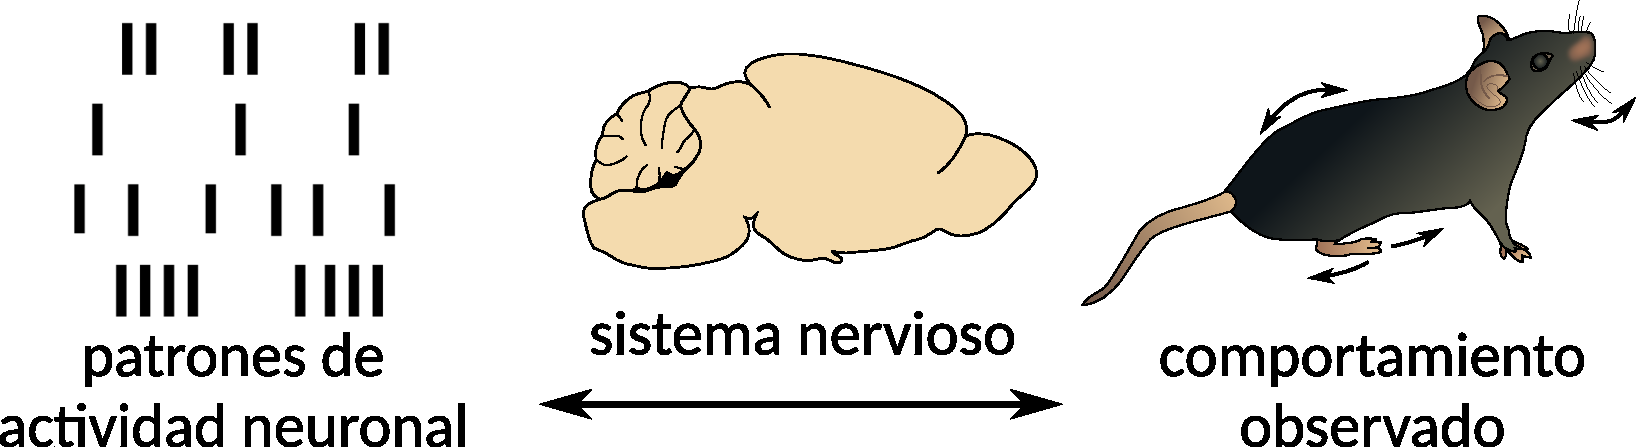
\includegraphics[width=0.6\linewidth]{figuras/introduccion/actividad_comportamiento.pdf}
    \caption{El estudio de las correlaciones entre la actividad neuronal y los comportamientos animales suscitados, puede ayudar a dilucidar el funcionamiento de diferentes regiones del sistema nervioso.}
    \label{fig:actividad_neuronal}
\end{figure}

El concepto de estereotipia tiene una gran utilidad cuando se trata de comprender cómo el cerebro controla dichos movimientos.
En este caso, la información resultante de la cuantificación del comportamiento es de fundamental importancia para su correlación con registros simultáneos de la actividad neuronal con el fin de estudiar cómo el cerebro codifica diferentes movimientos, cuáles son los circuitos neuronales subyacentes y cómo estos se modifican durante el aprendizaje de nuevas tareas motoras (Figura \ref{fig:actividad_neuronal}) \cite{esposito_defensive,levy_representation}. A pesar de su importancia, la determinación del repertorio de movimientos de un animal resulta experimentalmente complicada, debido a las dificultades que conlleva la cuantificación del comportamiento animal en términos objetivos y reproducibles.

En este trabajo nos proponemos explorar el espacio de comportamientos a los que accede un conjunto de ratones realizando una tarea de destreza motora de manera no supervisada. La tarea estudiada se denomina rotarod con aceleración, la cual consiste en entrenar ratones para que caminen sobre un cilindro que gira a velocidades crecientes, con aceleración constante. El \textit{rotarod} con aceleración es un paradigma experimental ampliamente utilizado en el estudio del aprendizaje motor dado que la \textit{performance} del animal mejora con el entrenamiento de manera dependiente de la plasticidad neuronal \cite{costa_motor_learning}. Sin embargo, el desempeño del animal en esta tarea se suele evaluar simplemente a través de la medición del tiempo de permanencia en el cilindro. En este contexto nos preguntamos, ¿cuáles son los cambios en el repertorio de movimientos del animal asociados a un mejor desempeño de la tarea? 

Para contestar esta pregunta realizamos una serie de filmaciones de los animales mientras realizaban la tarea motora. Para cuantificar los movimientos, se extrajeron coordenadas bidimensionales de las posiciones de algunas partes de sus cuerpos y su evolución en el tiempo. Para ello, se utilizó \textit{DeepLabCut}, un \textit{software} \textit{open-source} de \textit{motion-tracking}, que no requiere la utilización de marcadores físicos adicionales sobre los cuerpos de los animales \cite{mathis_deeplabcut}. A partir de estas coordenadas se calcularon posiciones relativas en función del tiempo. De esta manera, se extrajo información cuantitativa de las posiciones de los ratones y de sus partes del cuerpo durante el transcurso de la tarea \textit{rotarod}.

Para dilucidar la estructura intrínseca de este conjunto de datos se utilizó el algoritmo t-SNE para la reducción de la dimensión de manera no lineal \cite{vdm_tsne}. La transformada t-SNE es también una herramienta popular para la visualización de conjuntos de datos de dimensión alta y se utiliza frecuentemente en el ámbito de la bioinformática para visualizar datos provenientes de la secuenciación del material genético de células individuales \cite{kobak_art}. Así se construyó un mapa de comportamientos en 2 dimensiones donde se proyectan cada uno de nuestros vectores de dimensión mayor que describen la posición de los ratones y de sus partes del cuerpo.

Luego, procedimos a analizar la dinámica de transiciones en este espacio de dimensión reducida producido por el algoritmo t-SNE y se identificaron \textit{clusters} de puntos que se corresponden con poses específicas adoptadas por los ratones durante la ejecución de la tarea \textit{rotarod}. Así, se utilizó de manera efectiva al algoritmo t-SNE para la clasificación no supervisada de poses animales. Esta clasificación es robusta y representativa de nuestro conjunto de ratones estudiados ($N_{\mathrm{ratones}}=3$) y tiene potencial tanto como para reimplementarse utilizando un mayor número de ratones \textit{a priori}, como también para agregar nuevas observaciones experimentales al mapa t-SNE \textit{a posteriori} \cite{kobak_art, korsunsky_harmony}. Interpretaremos entonces como comportamientos estereotipados a diferentes sucesiones de estas poses clasificadas. En particular, nos concentraremos en el estudio de transiciones de primer orden entre dos poses distintas, pero también exploraremos la dinámica de transiciones de poses a escalas de tiempo mayores.

En simultáneo, durante la ejecución de la tarea \textit{rotarod}, se registró la actividad de neuronas individuales de la región locomotora del mesencéfalo (MLR) de los ratones ya entrenados en la tarea. El MLR es una región implicada en los procesos de iniciación y de control de la velocidad de la locomoción \cite{caggiano_midbrain, roseberry_locomotor, shik_walking}. Por lo tanto, en este experimento nos preguntamos si la actividad de algunas de las neuronas presentes en esta región del cerebro estaría modulada por el movimiento del ratón en el transcurso de la tarea \textit{rotarod} \cite{skinner_mlr_rat, sherman_mlr_cat, leray_mlr_vertebrate}. Para contestar esta pregunta correlacionamos la actividad neuronal con la ocurrencia de transiciones entre poses específicas obtenidas a partir de la clasificación no supervisada del comportamiento. Este estudio nos permitió demostrar la existencia de neuronas en el MLR (alrededor de un cuarto del total de neuronas registradas) cuya actividad neuronal varía significativamente alrededor de las transiciones entre poses clasificadas. Este resultado sugiere fuertemente que el MLR no solo codificaría la iniciación y la velocidad de la locomoción sino también el tipo de movimiento seleccionado.

\thispagestyle{empty}